\documentclass[12pt]{article}
\usepackage[english]{babel}
\usepackage{graphicx, color, xcolor, wrapfig, subcaption}
\usepackage{amsmath}
\usepackage{hyperref}
\usepackage{verbatim}
\usepackage{algorithmic}
\usepackage{algorithm}

%\usepackage{tabularx}
\usepackage{booktabs}
\usepackage{siunitx}
\usepackage{float}

\graphicspath{ {images/} }
\hypersetup{
    colorlinks,%
    citecolor=green,%
    filecolor=magenta,%
    linkcolor=red,%
    urlcolor=cyan
}

\title{CS531 Programming Assignment 2: Towers of Corvallis}
\author{
        Santosh Kumar, Daniel Magee \\
        (EECS, MIME), Oregon State University\\
}
    
\begin{document}

\maketitle

\begin{abstract}
In this project, we examine two informed search algorithms, Astar and Beam search, using admissible and non-admissible heuristics to solve a variant of the well-known tower of Hanoi problem. 
We were able to complete each run up to $10$ disks within a maximum time of~\SI{1.5}{min}.
We found that Beam search significantly outperformed Astar on runtime for the beam width we chose.
\end{abstract}
    
\section{Introduction}
In this formulation of the well known towers of Hanoi puzzle, the towers of Corvallis, the environment consists of three poles and some number of disks with distinct, integer radii.
Unlike the towers of Hanoi, in our case any disk can rest on top of any other disk. 
One disk, on the top of a tower, may be moved each turn.
The problem begins with all disks on the first pole in arbitrary order.
The solution is the path to the goal, all the disks sorted in ascending order.

We compare two informed search algorithms and two heuristics, admissible and non-admissible, to explore the decision tree and find the path to the goal.
The aim is to find the shortest path to the goal while expanding the fewest nodes possible.

\section{Algorithms}
\begin{algorithm}[!h]
\caption{Path Reconstruction}
\label{alg:reconstructpath}
\begin{algorithmic}
\STATE function solutionPath(state):
\STATE solvedPath=[state]
\WHILE{state in path}
	\STATE previousState = path[state]
	\STATE state = previousState
	\STATE solvedPath.append(state)
\ENDWHILE
\RETURN solvedPath
\end{algorithmic}
\end{algorithm}

\subsection{Astar}
Algorithm~\ref{astar} describes Astar search, a type of best-first search which uses a heuristic to gauge the distance to the goal, $h$, and adds it to the path cost, $g$, to choose the next node to expand, that is, the direction that seems most likely to reach the goal first.
Astar uses a priority queue implemented on a heap to sort the best potential nodes on the frontier.
The heap stores tuples for each frontier node which take the form $(heuristic cost ~ [g + h], g, [frontierState.parent, frontierState])$.
When a node is chosen, it is removed from the queue and added to the \textit{path} where the node is the key an the parent is the value (the parent is already a key in the map pointing to it's parent).
When we find the goal, we travel up the map collecting the path using the path reconstruction function given in Algorithm~\ref{alg:reconstructpath}.

\begin{algorithm}[!h]
\caption{Astar Search}
\label{astar}
\begin{algorithmic}
\STATE function Astar(state, heuristicType):
\STATE Q:=heapify(state)
\IF{state is goal state}
	\RETURN \textit{solutionPath(state)}
\ENDIF
\IF{disk is not last moved}
    \STATE successors = move disks column top disks
    \STATE cost = \textit{heuristic(successors)}
\ENDIF 
\FOR{s in successors}
    \IF{s in Q}
        \STATE keep s with min cost
    \ELSIF{s in \textit{path.keys()}}
        \STATE delete s
    \ELSE
        \STATE Q.push(s)
    \ENDIF
\ENDFOR

\IF{Q is empty}
	\RETURN failure
\ELSE
	\STATE minQ := Q.pop()
    \STATE path.Add(minQ: minQ.parent)
    \RETURN minQ
\ENDIF
\end{algorithmic}
\end{algorithm}


\subsection{Beam Search}
\begin{algorithm}[!h]
\caption{Beam Search}
\label{Beam}
\begin{algorithmic}	
\STATE function Astar(state, beamWidth, heuristicType):
\STATE Q:=heapify(state)
\IF{state is goal state}
	\RETURN \textit{solutionPath(state)}
\ENDIF
\IF{disk is not last moved}
	\STATE successors = move disks column top disks
	\STATE cost = \textit{heuristic(successors)}
\ENDIF 
\FOR{s in successors}
\IF{s in \textit{path.keys()}}
	\STATE delete s
\ELSIF{s in \textit{path.keys()}}
	\STATE keep s with min cost
\ELSE
	\STATE Q.push(s) 
\ENDIF
\ENDFOR
	
\IF{Q is empty}
	\RETURN failure
\ELSE
	\FOR{i in 1:beamWidth}
		\STATE mQ.append(Q.pop())
		\STATE path.Add(s: s.parent)
	\ENDFOR
	\RETURN mQ
\ENDIF
	\end{algorithmic}
\end{algorithm}

Beam search is described by Algorithm~\ref{Beam}.  
Beam search uses the same heuristics as Astar; however, instead of maintaining a frontier across tree depths and between expansions, it pushes to a size-limited sorted heap and pops the entire queue after every turn.
The size of the frontier is limited by the beam width parameter.
Since the queue is emptied and repopulated every turn, all frontier nodes exist at the same depth.
Beam search maintains a map creating links from children to parent nodes as they are expanded.  
This mapping provides a way to reclaim the path and a set of all previously visited nodes which we use to exclude current child nodes from the queue.

\section{Heuristics}

Without heuristics informed searches are simply uniform cost searches.
There are no universally effective heuristics, although there are some, such as Manhattan distance, that are generally effective in a wide range of applications.

Initially, we explored using the Manhattan distance as a heuristic for this problem, but it was not effective.
Unlike seemingly similar problems, such problem 3.27 in the text (where the cars must cross each other to reach their destination, the towers of Corvallis does not exist in an environment with a static shape.
Since moving the disks changes the distance of all the other blocks to their goal, and makes the goal of some blocks a non-existent placement above a column, the Manhattan distance is ambiguous.

The towers of Corvallis is similar to the towers of Hanoi in that solving a tower of $n$ disks is identical to solving a tower of a single disk $n$ and subsequently solving $n-1$ disks.
This leads to our guiding principle: once the single largest disk is solved for, it is catastrophic for it to be moved.
Thus our admissible heuristic is exceedingly simple: $h(n) = max(d_{misplaced}) + n_0/n_{total}$.
This returns the maximum value disk that is not in it's goal position added to the proportion of all disks on the first tower.
It might be said that this is not an admissible heuristic since the shortest possible path to the final would be $max(d_{misplaced})$ as the subsequent disks are added to the tower.
However, the proportion of disks on the first column is fractional, and, since all other values are integers, solves only as a tiebreaker between otherwise equivalent heuristics.
We contend that this qualifies the heuristic as, at least, conditionally admissible.

Our non-admissible heuristic simply squares $max(d_{misplaced})$.

\section{Results}

Our experiments evaluated twenty initial arrangements of disks on the first tower for Beam search with $beam width=10$ and Astar search for both heuristics.
The experiments were evaluated using an Intel Xeon E5-2630 2.4 GHz processor and were executed in serial.
All programs are written in python and contain no interruptive mechanisms, so cpu and wall clock time are synonymous.

\subsection{Beam Width Optimality}

First, we executed Beam search with a limited selection of initial conditions.  
We averaged the results for each $n$ problem size.
As shown in the figures below, beam search was able to find a solution to the puzzle in less than half a minute for all problem sizes, heuristics, and widths.

\begin{figure}[H]
	\centering
    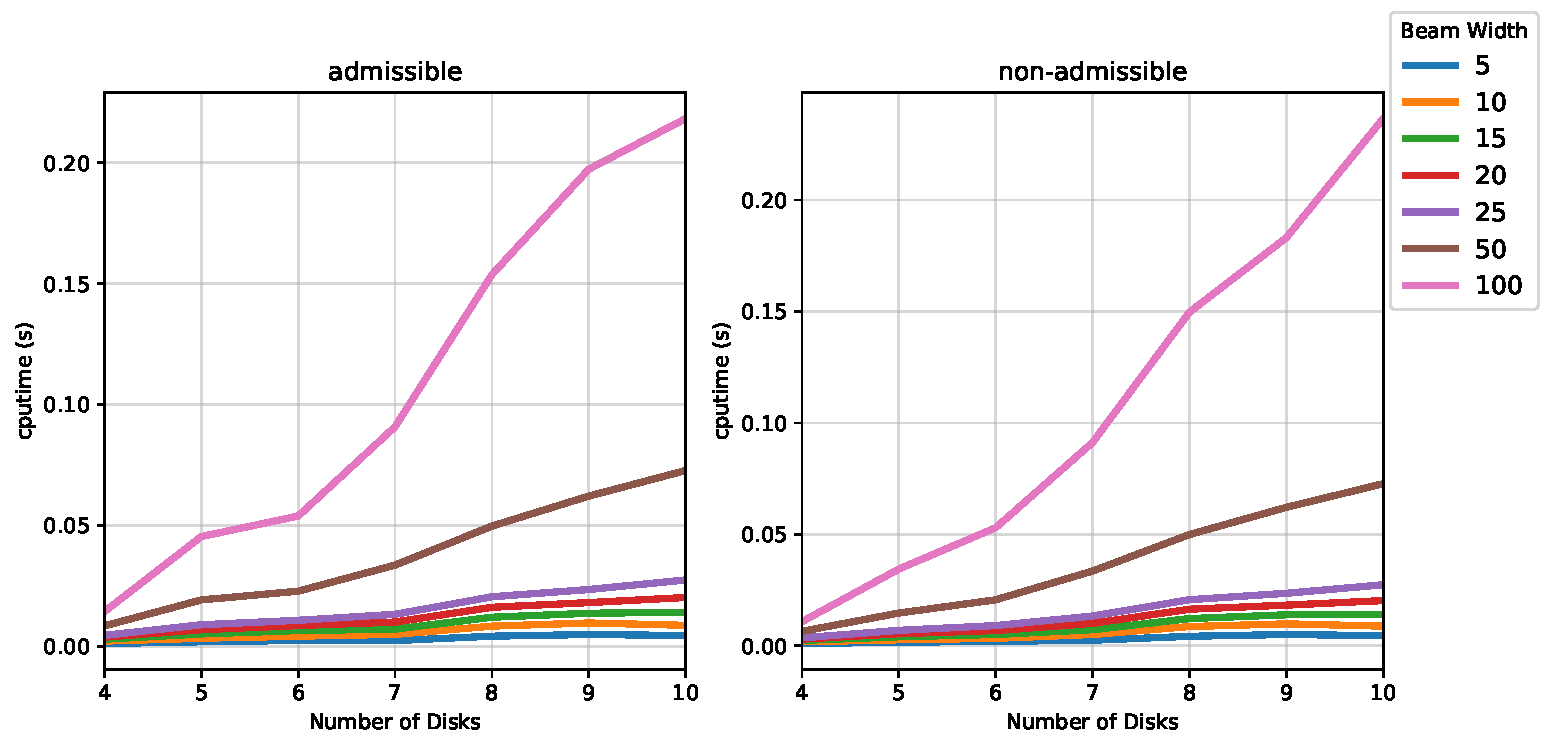
\includegraphics[width=\textwidth]{BeamTestCputime}
	\caption{Time to solution for Beam search with various widths.}	
	\label{f:BeamCpu}
\end{figure}
\begin{figure}[H]
	\centering
    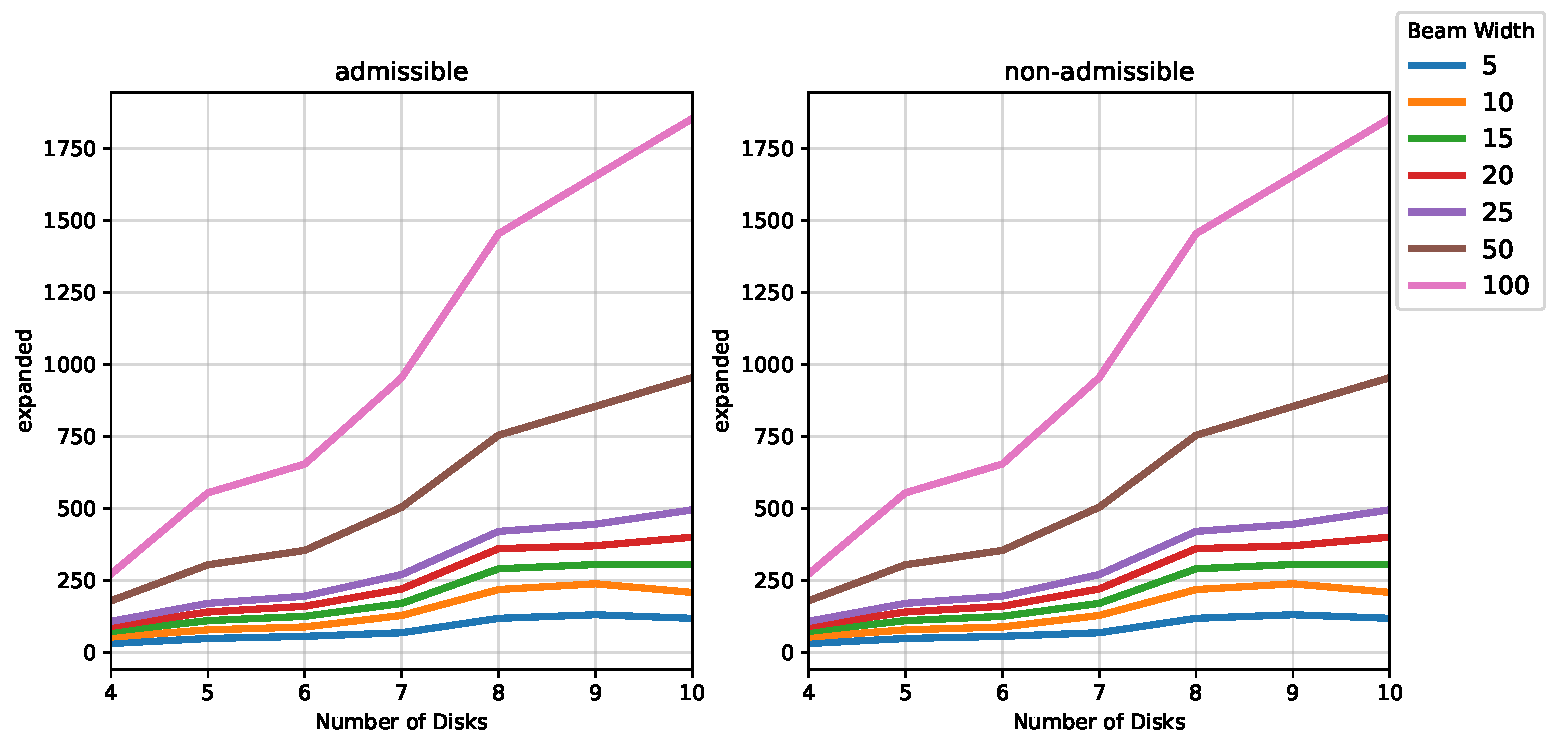
\includegraphics[width=\textwidth]{BeamTestExpanded}
	\caption{Number of nodes expanded by Beam search.}
	\label{f:BeamEx}
\end{figure}
\begin{figure}[H]
	\centering
    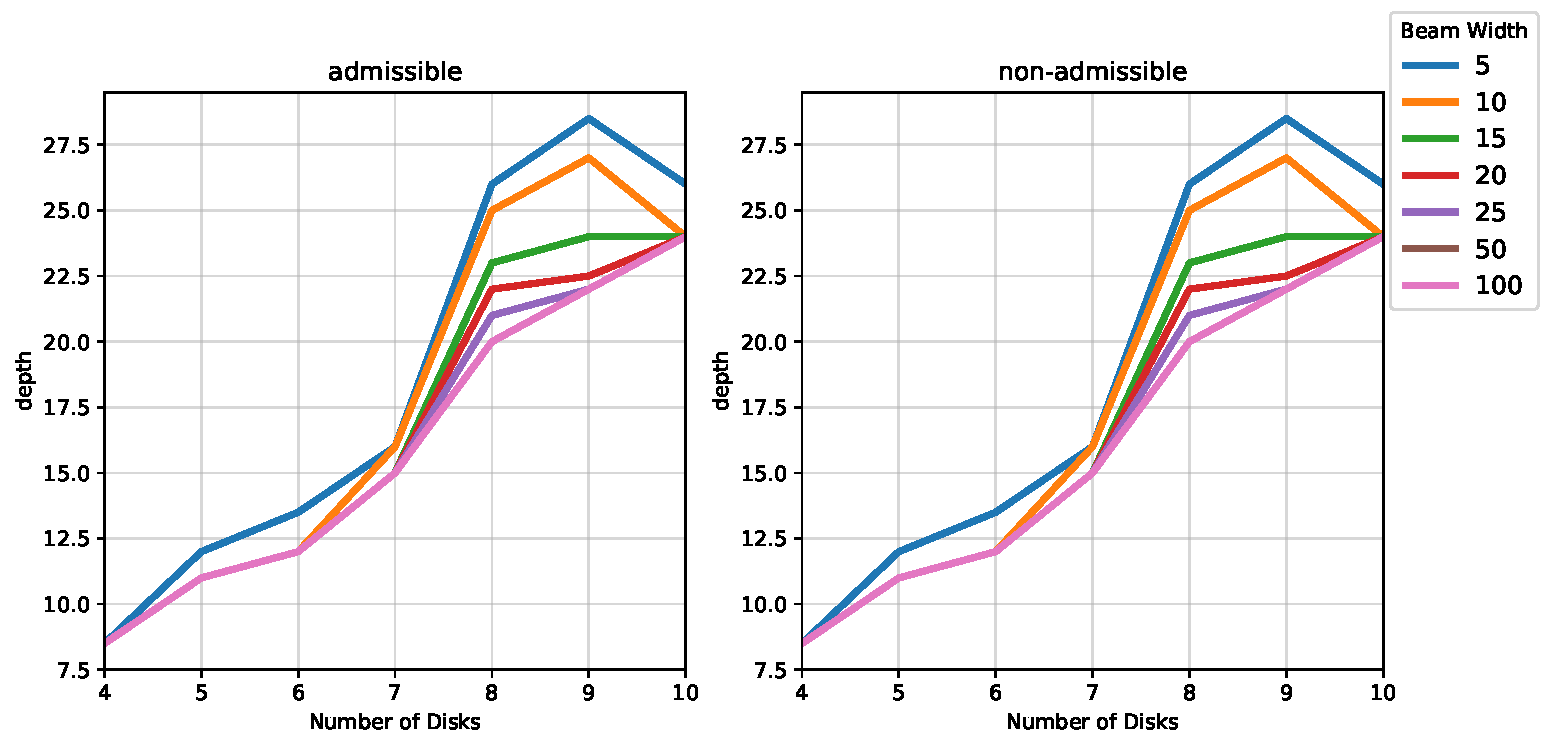
\includegraphics[width=\textwidth]{BeamTestDepth}
	\caption{Depth of solution found by Beam search.}
	\label{f:BeamDepth}	
\end{figure}

Beam search presents a trade-off between accuracy (optimality) and speed.
The deleterious effects of a narrow beam can be seen clearly in Figure~\ref{f:BeamDepth}.
Beams of widths 5 and 10 find solutions with significantly longer path lengths than beams with widths 25-100 at problem size 9.
They do this far more quickly, Figure~\ref{f:BeamCpu}, while expanding far fewer nodes, Figure~\ref{f:BeamEx}.
Examining these results, we decided that a beam width of 10 is provides a good balance, it finds the same solutions as width 100 for problem sizes of $4,5,6,10$ and is significantly faster.

\subsection{Algorithm Comparison}

After deciding on a standard beam width, we ran all the test conditions for Beam and Astar search for both heuristics.
The following plots show the runtime, solution depth, and number of expanded nodes for all search types and heuristics.

\begin{figure}[H]
	\centering
    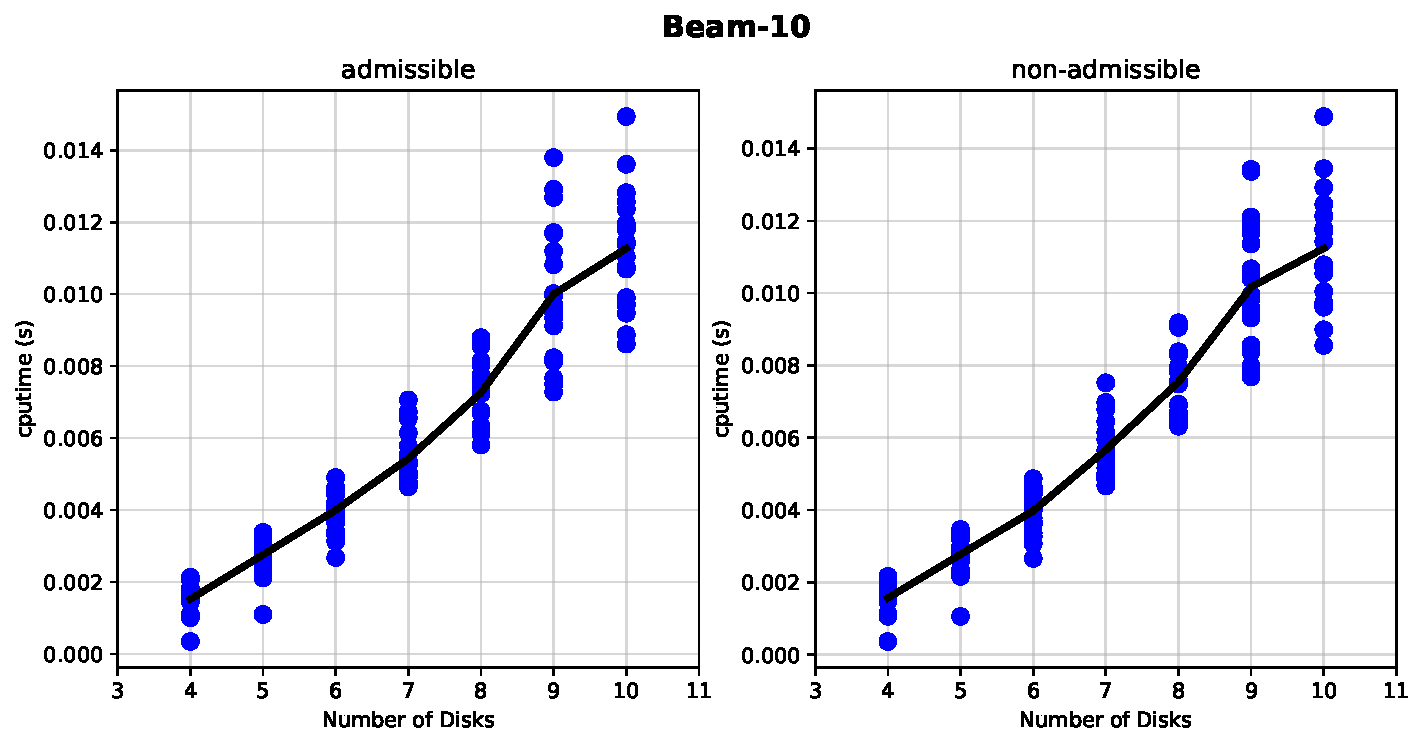
\includegraphics[width=.9\textwidth]{FullCputimeBeam-10}	
	\caption{Runtime of Beam search at all test conditions. Line shows average at each problem size}
	\label{f:FullCpuBeam}
\end{figure}
\begin{figure}[H]
	\centering
    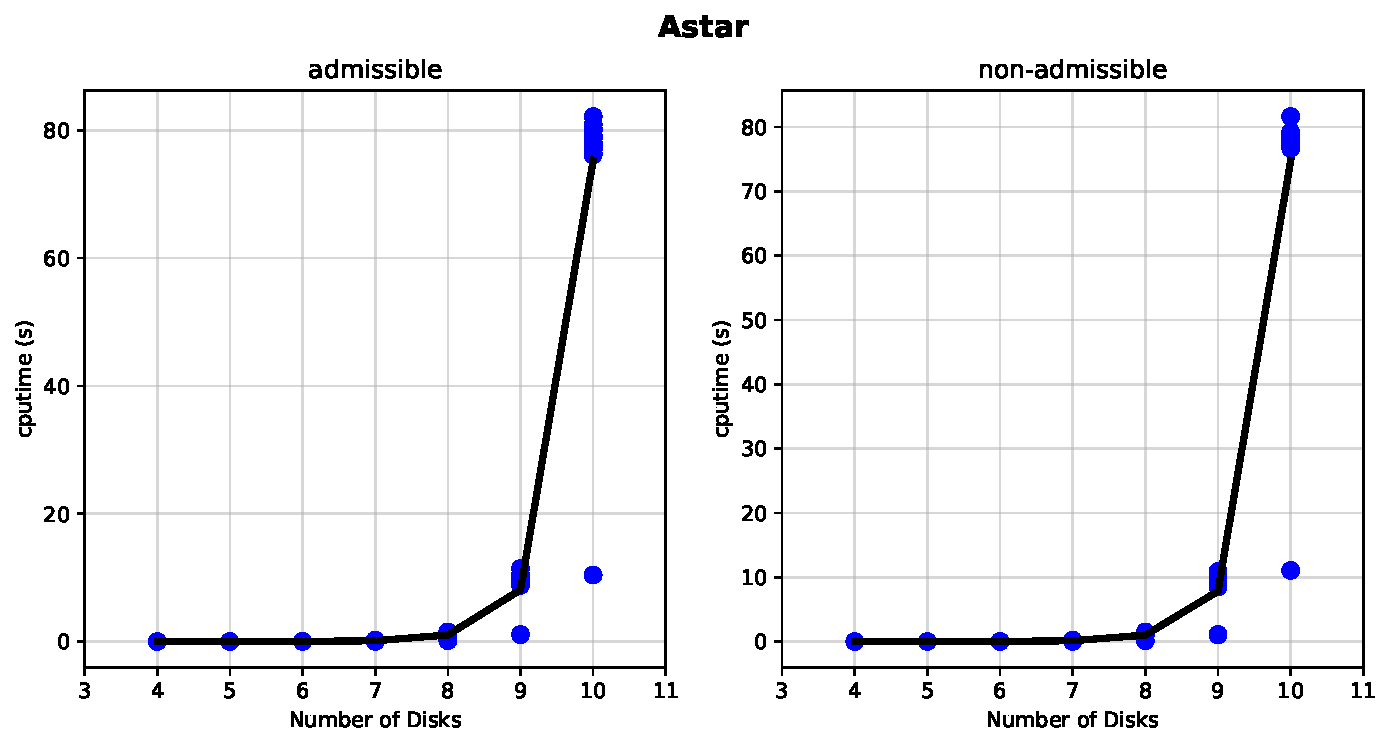
\includegraphics[width=.9\textwidth]{FullCputimeAstar}	
	\caption{Runtime of Astar search at all test conditions. Line shows average at each problem size}
	\label{f:FullCpuA}
\end{figure}

Comparing the runtimes, the metric that really matters, of Astar and beam search shows Beam search with a significant edge.
Beam search scales linearly while Astar scales exponentially.
These Figures~\ref{f:FullCpuBeam}~\ref{f:FullCpuA} also show that the heuristics have little impact on the time cost of the searches. 
There does seem to be a slightly perceptible improvement in Astar using the non-admissible heuristic.

\begin{figure}[H]
	\centering
    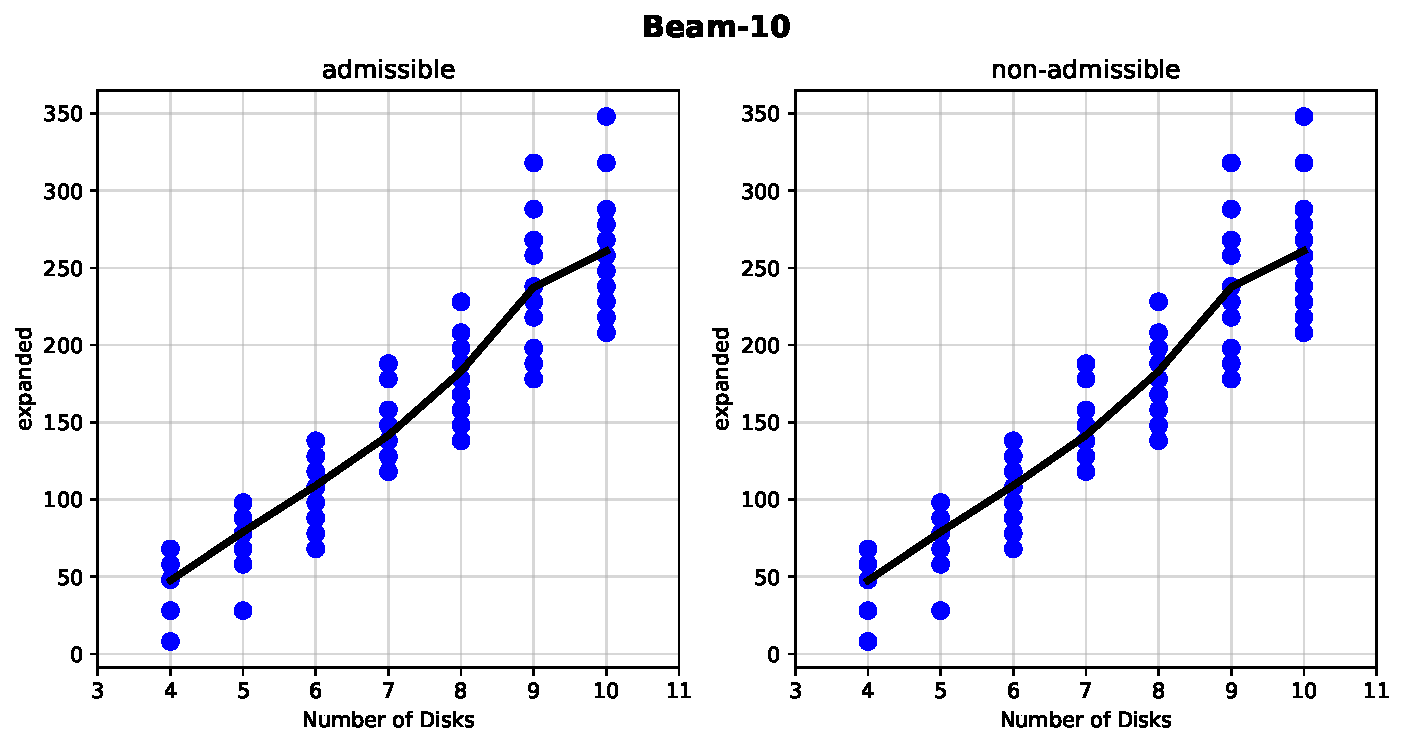
\includegraphics[width=.85\textwidth]{FullExpandedBeam-10}	
	\caption{Beam search width 10 number of nodes expanded.}
	\label{f:FullExBeam}
\end{figure}
\begin{figure}[H]
	\centering
    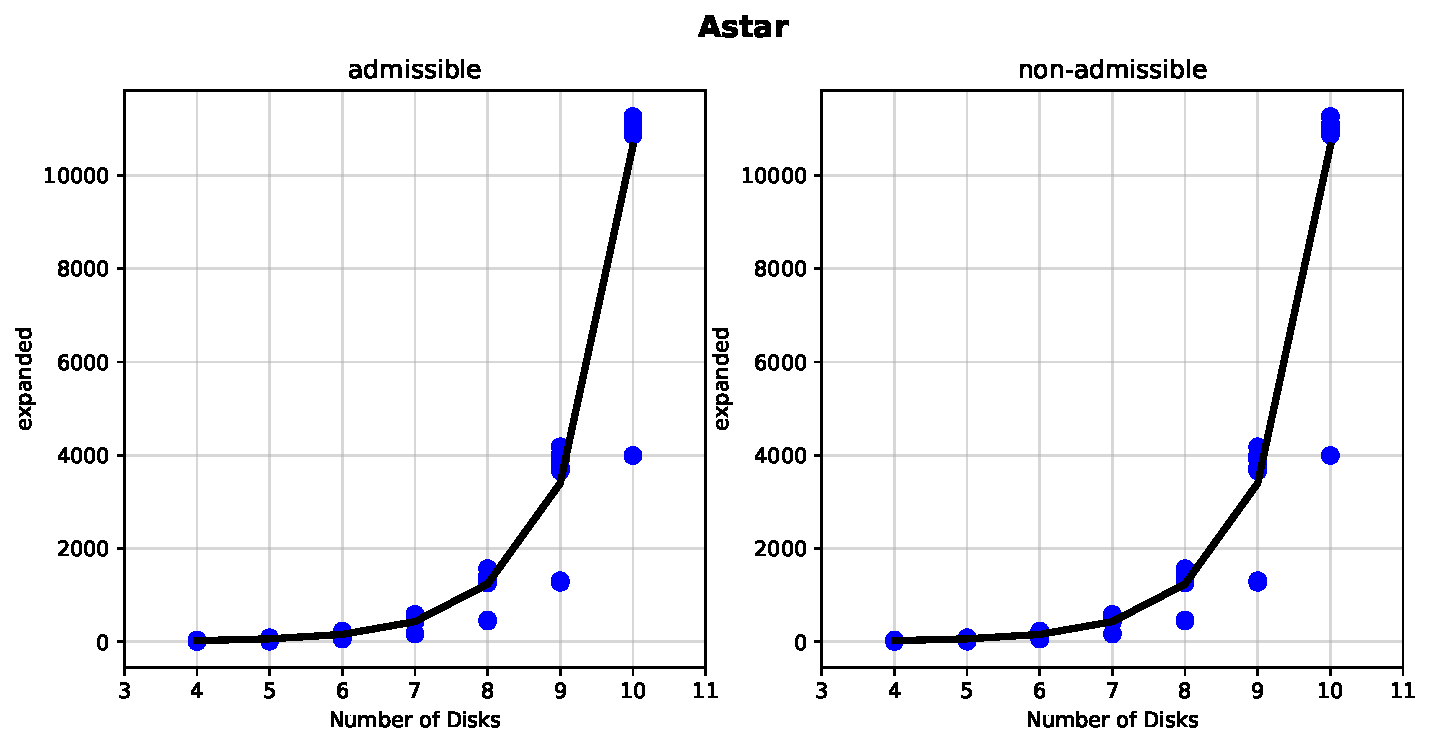
\includegraphics[width=.85\textwidth]{FullExpandedAstar}
	\caption{Number of nodes expanded in Astar search.}
	\label{f:FullExA}	
\end{figure}

The reason Beam search is able to achieve such performnce improvements is the way that the number of expanded nodes scales slowly and linearly with problem size.
This is intuitive since beam search can only visit width number of nodes at each depth whereas the multi-depth frontier of Astar is able to grow at a super-linear rate as it spreads over deeper paths. 
The existence of under-average outliers, markedly clear in Astar, underscores the earlier observation relating to heuristics.
That is: solving a problem with $n$ disks is identical to solving the problem for a single disk $n$ and then solving an $n-1$ problem.
These outliers cost the same as a problem of size $n-1$ because the initial condition places the largest disk in the correct place.

\begin{figure}[H]
	\centering
    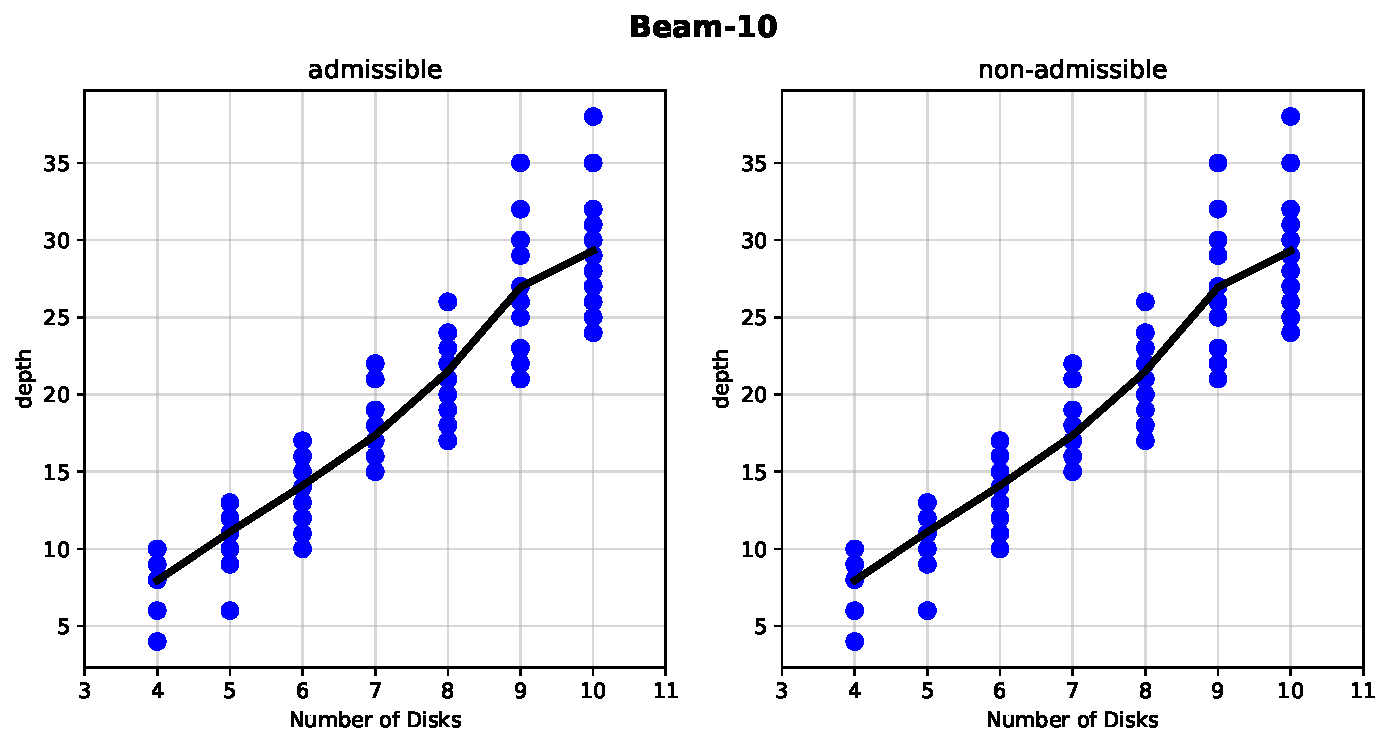
\includegraphics[width=.8\textwidth]{FullDepthBeam-10}	
	\caption{Solution depth for Beam search}
	\label{f:FullBeamDepth}
\end{figure}
\begin{figure}[H]
	\centering
    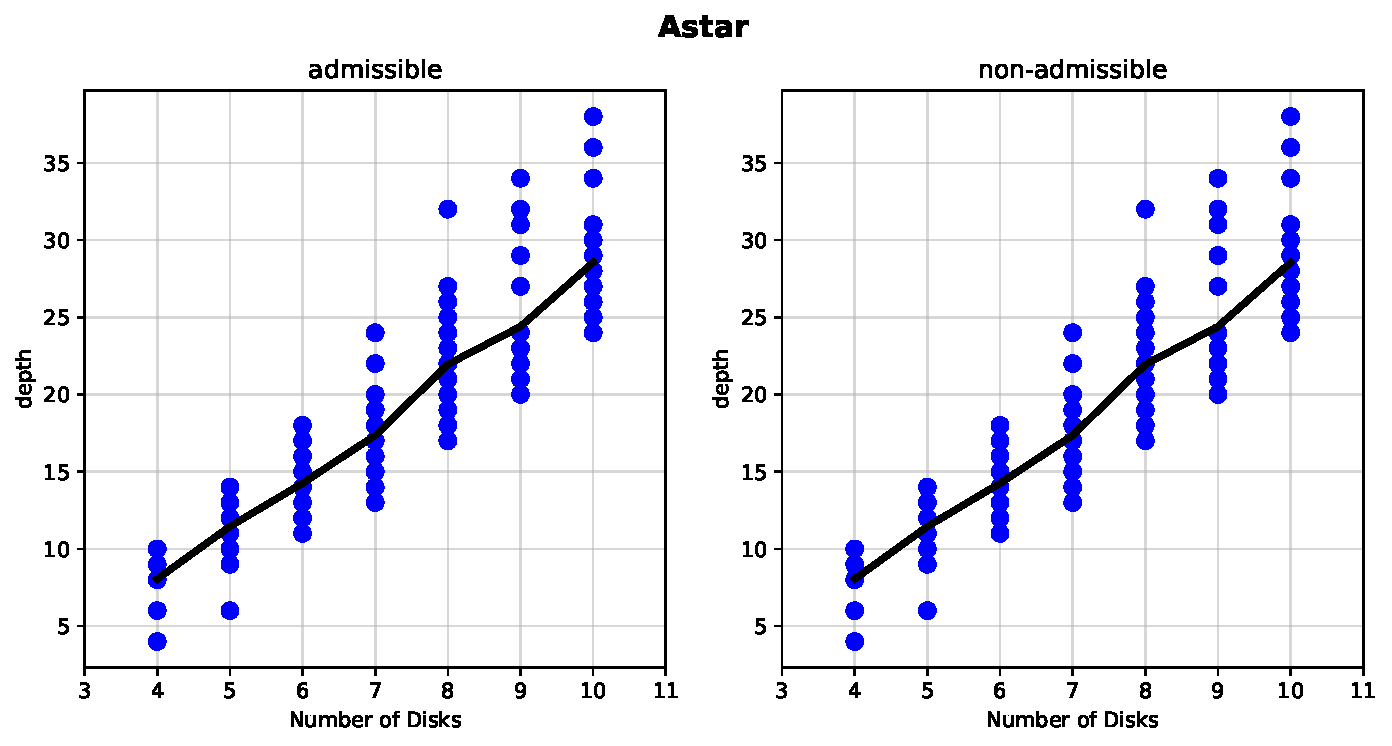
\includegraphics[width=.8\textwidth]{FullDepthAstar}	
	\caption{Solution depth for Astar search}
	\label{f:FullADepth}
\end{figure}

Lastly, Astar and Beam search find similar solutions at similar depths.  
There is a distribution, and it seems like Astar performs slightly better overall, but the differences are minor.

\section{Discussion}

\textbf{1. Show an example solution sequence for each algorithm for the largest size you tested in the following format}.
NOTE: Our solutions are calculated and shown with the opposite orientation (top disk is rightmost).  
Conceptually this makes it a FIFO queue which is more efficient for pushing and popping.  
In addition, the results are strings in tuples rather than digits in lists as shown.

The initial condition for all of these results is a disk ordering of \textit{3685790124} on the first disk. 
The path length for the Astar and Beam solutions are 31 and 32 respectively and there is no difference in the solution due to the heuristics, so only one solution is shown for each.  
The beam width is set at 10, which we determined as the best balance of accuracy and performance based on our initial experiment on beam width.

\textbf{Astar}
\begin{verbatim}
('9876543210', '', '')
('987654321', '0', '')
('98765432', '01', '')
('9876543', '01', '2')
('9876543', '0', '21')
('987654', '03', '21')
('987654', '031', '2')
('987654', '0312', '')
('98765', '0312', '4')
('98765', '031', '42')
('98765', '03', '421')
('98765', '0', '4213')
('9876', '05', '4213')
('987', '05', '42136')
('987', '0', '421365')
('98', '07', '421365')
('98', '075', '42136')
('9', '0758', '42136')
('9', '07586', '4213')
('9', '075863', '421')
('', '075863', '4219')
('3', '07586', '4219')
('36', '0758', '4219')
('368', '075', '4219')
('3685', '07', '4219')
('36857', '0', '4219')
('368579', '0', '421')
('3685790', '', '421')
('36857901', '', '42')
('368579012', '', '4')
('3685790124', '', '')
\end{verbatim}

\textbf{Beam}
\begin{verbatim}
('9876543210', '', '')
('987654321', '0', '')
('98765432', '01', '')
('9876543', '01', '2')
('9876543', '0', '21')
('987654', '03', '21')
('987654', '031', '2')
('987654', '0312', '')
('98765', '0312', '4')
('98765', '031', '42')
('98765', '03', '421')
('98765', '0', '4213')
('9876', '05', '4213')
('9876', '053', '421')
('987', '0536', '421')
('98', '0536', '4217')
('9', '05368', '4217')
('9', '053687', '421')
('', '053687', '4219')
('', '05368', '42197')
('', '0536', '421978')
('', '053', '4219786')
('3', '05', '4219786')
('36', '05', '421978')
('368', '05', '42197')
('3685', '0', '42197')
('36857', '0', '4219')
('368579', '0', '421')
('3685790', '', '421')
('36857901', '', '42')
('368579012', '', '4')
('3685790124', '', '')
\end{verbatim}

\textbf{2. How did the search time and the solution quality vary with the beam width? Is there a beam width that gives the best trade-off for the two heuristics?}

Smaller beam widths give better CPU times but may not converge as the quality of solution diminishes with increasing number of nodes excluded from the search. On running the simulations multiple times, we found that beam width=10 gives same performance to the ones slightly higher/lower than that for similar CPU time and no. of nodes expanded for varying $n$ values.

\textbf{3. How did the search time and the solution quality vary with the beam width? Is there a beam width that gives the best trade-off for the two heuristics?}

The Beam search algorithm significantly outperformed the A* search for larger values of $n$ in terms of number of nodes expanded and the runtime in case of first heuristic but the second heuristic reduction of the runtime and number of nodes expanded are less in no. upon comparison with reduction for the A* search.

\textbf{4. Can a small sacrifice in optimality give a large reduction in the number of nodes expanded? What about CPU time?}

Yes, If instead of reaching the goal state, we stop where the heuristic is like,say 2 i.e. it is 2 state different from becoming the optimal[final] solution.
For 0123456789, the final state is 9876543210 but if we get 9786543210, it is 2 steps away from optimal, we can stop here which reduces the number of steps and the CPU time for every case as all the nodes need not be expanded from here on out, significantly improving the performance of A* and beam search by a factor.

\textbf{5. Can a small sacrifice in optimality give a large reduction in the number of nodes expanded? What about CPU time?}
We considered the Admissible Manhattan distance as it is one of the standard heuristic functions used in AI, while the heuristic gives a good estimate, it is very slow and takes a lot of steps to converge. 

The sacrifice of optimality for other performance metrics is shown well in Figures~\ref{f:BeamCpu},~\ref{f:BeamDepth}. 
They show how 

\textbf{6. How do the two algorithms compare in the amount of search involved and the cpu-time?}

A* Search is complete in the sense that it searches all the possible nodes, while the Beam search prunes the higher heuristic value nodes so it only searches for the least cost solution. 
That is, it makes a permanent decision upstream about the avenues it will pursue to find the solution whereas A* keeps options that look terrible right now open for consideration.
A* search searches all the nodes which significantly increases the CPU time as all the nodes are expanded, Beam search searches only lower heuristic value nodes as it expands the lower cost nodes for some beam width, so the CPU time in the Beam Search algorithm is lower than A* search for higher values of n(no. Of disks).

\textbf{7. Do you think that either of these algorithms scale to even larger problems? What is the largest problem you could solve with the best algorithm+heuristic combination? Report the wall-clock time, CPU-time, and the number of nodes searched.}

The Beam Search scales well for larger problems using the non-admissible heuristic. The largest problem we solved for this project is of size n=10, “0123456789” with solution as “9876543210” where we found the no. of nodes to be expanded as 208 with length of solution= 24 and runtime equal to 0.0139797926. 

We did experiment with larger problems. Currently running the Corvallis.py file will launch a problem with size $n=50$. On a mediocre laptop, this completed in .2 seconds.  So we imagine that it could go much higher. 
If the linear trend shown in Figure~\ref{f:FullCpuBeam} scaled infinitely, we estimate that runtime would reach \SI{10}{mins} at about $n=400000$.

The best algorithm would have to be Beam search with a relatively narrow beam, and the non-admissible heuristic.

\textbf{8. Is there any tradeoff between how good a heuristic is in cutting down the number of nodes and how long it took to compute? Can you quantify it?}

Yes, if we want the best possible heuristic which considers all the possible cases/nodes it would take a lot of time to evaluate the heuristic but it will definitely give the optimal solution given the Nmax[max. Nodes expanded] is large enough. Otherwise, if the best possible heuristic is not considered, we may sacrifice optimality of the solution or the completeness of the solution as we do not consider all the possibilities/paths from all the nodes but it would converge faster if only a subset of the few best nodes in the frontier are expanded.

Hence, goodness of heuristic is directly proportional to the number of nodes and inversely proportional to the time taken to compute the solution (sequence).

\textbf{9. Is there anything else you found that is of interest?}

It was surprising to see that A* performs equally well in comparison to Beam search for lower beam width values for smaller n, because even though the value of n was lower, I expected beam search to outperform A*, maybe it was because the values of n are so small which led to lesser number/depth of paths which didn`t hinder the performance of A*.

\end{document}